\documentclass[12pt,twoside]{report}
\usepackage[a4paper,width=150mm,top=25mm,bottom=25mm,bindingoffset=6mm]{geometry}
\usepackage[english]{babel}

\setlength{\headheight}{15pt} 

\usepackage[utf8]{inputenc}
%\usepackage[latin1]{inputenc}
\usepackage{fancyhdr}
\usepackage{indentfirst}
\usepackage{graphicx}
\graphicspath{ {Images/}  }
\usepackage{newlfont}
\usepackage{amssymb}
\usepackage{amsmath}
\usepackage{latexsym}
\usepackage{amsthm}
\usepackage{listings}
\usepackage{xcolor}
\usepackage{mdframed}
\usepackage{epigraph}
\usepackage{csquotes}


\usepackage{breqn}

\usepackage[backend=biber]{biblatex}
\addbibresource{references.bib}

%\usepackage{array}
%\usepackage{tabu}

\usepackage{amsmath}
\usepackage{amssymb}


\usepackage{lipsum}

%\usepackage{pgf-pie}


%\usepackage{pgfplots}

%\pgfplotsset{
 % compat=newest,
  %xlabel near ticks,
 % ylabel near ticks
%}

\pagestyle{fancy}\addtolength{\headwidth}{20pt}
\renewcommand{\chaptermark}[1]{\markboth{\thechapter.\ #1}{}}
\renewcommand{\sectionmark}[1]{\markright{\thesection \ #1}{}}
\rhead[\fancyplain{}{\bfseries\leftmark}]{\fancyplain{}{\bfseries\thepage}}
\cfoot{}
\linespread{1.3}  
\begin{document}



\begin{titlepage}               

\thispagestyle{empty}                  
\topmargin=6.5cm                        
\raggedleft                            	
\large                                 		
\em                                    
%Questa \`e la \textsc{Dedica}:\\
%ognuno pu\`o scrivere quello che vuole, \\
%anche nulla \ldots     
INTA 'NA SAMANA NASCE 'NU ZITEDU E DICE: CIAO PAPA!
\newpage                            
\clearpage{\pagestyle{empty}\cleardoublepage}
\end{titlepage}
\pagenumbering{roman}                   
\chapter*{Abstract}             
\rhead[\fancyplain{}{\bfseries
Abstract}]{\fancyplain{}{\bfseries\thepage}}
\lhead[\fancyplain{}{\bfseries\thepage}]{\fancyplain{}{\bfseries
Abstract}}

%%%%%%%%%%%%%%%%%%%%%%%%%%%%%%%%%%%%%%%%%aggiunge la voce Introduzione
                                        %   nell'indice
\addcontentsline{toc}{chapter}{Abstract}
%\input{Introduction}
%%%%%%%%%%%%%%%%%%%%%%%%%%%%%%%%%%%%%%%%%non numera l'ultima pagina sinistra
\clearpage{\pagestyle{empty}\cleardoublepage}

%\rhead[\fancyplain{}{\bfseries\thepage}]{\fancyplain{}{\bfseries
%INDICE}}
\rhead[\fancyplain{}{\bfseries\leftmark}]{\fancyplain{}{\bfseries\thepage}}
\lhead[\fancyplain{}{\bfseries\thepage}]{\fancyplain{}{\bfseries
INDICE}}
\tableofcontents                        %crea l'indice
%%%%%%%%%%%%%%%%%%%%%%%%%%%%%%%%%%%%%%%%%imposta l'intestazione di pagina


%%%%%%%%%%%%%%%%%%%%%%%%%%%%%%%%%%%%%%%%%non numera l'ultima pagina sinistra
\clearpage{\pagestyle{empty}\cleardoublepage}
\listoffigures                          %crea l'elenco delle figure
%%%%%%%%%%%%%%%%%%%%%%%%%%%%%%%%%%%%%%%%%non numera l'ultima pagina sinistra
\clearpage{\pagestyle{empty}\cleardoublepage}
\listoftables                           %crea l'elenco delle tabelle
%%%%%%%%%%%%%%%%%%%%%%%%%%%%%%%%%%%%%%%%%non numera l'ultima pagina sinistra
\clearpage{\pagestyle{empty}\cleardoublepage}
%%%%%%%%%%%%%%%%%%%%%%%%%%%%%%%%%%%%%%%%%imposta l'intestazione di pagina


\lhead[\fancyplain{}{\bfseries\thepage}]{\fancyplain{}{\bfseries\rightmark}}

\pagenumbering{arabic}                  %mette i numeri arabi


\chapter{Background}

In this chapter we are going to present the existing Cowbird framework realized within the SWAN project \cite{swanonline}. Cowbird is a flexible and energy efficient framework for building Android application that use both smartphone sensors and IoT sensors\cite{cowbirdarticle}. Cowbird extends the SWAN framework \cite{swanphd} and it supports context-based expressions (queries) that can run both on a smartphone and in the cloud; with the Cowbird framework, developers can easily decide where to perform the computation according to the source of the data and the frequency of the updates.

\section{The SWAN framework}
SWAN (Sensing With Android Nodes) is a framework for easily building context-aware applications for Android smartphones \cite{swanphd}. The framework provides application developers a high-level abstraction for accessing smartphone's sensors. In particular, the SWAN framework is designed to be executed as an Android background service and it acts as a middleware between applications and sensors: running applications can access it through a well-defined API. The SWAN framework reduces storage redundancy and code duplication caused by multiple sensor-based applications running simultaneously. In fact, it provides a centralized solution for collecting and storing data from sensors. 

\subsection{SWAN sensors}
One of the most important characteristic of SWAN is its \emph{multi sensor support}; in fact, at the moment, SWAN supports more than 20 different types of sensors. We can distinguish two different categories of sensors:
\begin{itemize}
\item	 \emph{Hardware sensors}. The physical sensors installed on the devices (e.g. accelerometer, GPS, etc.).
\item \emph{Software sensors}. Software \emph{data sources} (e.g. calendar, rain prediction, Twitter, etc.) that can be installed on the devices or that can run somewhere else. 
\end{itemize}

SWAN sensors are implemented as background services that are responsible for gathering the sensor's data. In case of external software sensors such as the rain prediction or Twitter, the SWAN sensor continuously polls from the web endpoint to get live data. The data accuracy can be improved increasing the polling frequency. 

From an architectural point of view all the SWAN sensors run in separate processes in order to remain unaffected if the application built on top of SWAN crashes: this design approach prevents data losses. The communication between SWAN sensors and the other components is performed through inter-process communication (IPC).

\subsection{SWAN-Song}
One of the SWAN framework core functionalities is the SWAN-Song support. SWAN-Song \cite{swansong} is a a domain specific language
for context expressions. SWAN-Song is used by applications to register expressions into SWAN. After registering an expression, SWAN evaluates it and sends back the result to the application. 

The SWAN-Song language is a form of zeroth-order logic, which allows the description of a particular combination of contextual information using sensor based expression predicates. Predicates can be combined using math, comparison, and logic operators, and a specification of a \emph{history window} and \emph{history reduction} operator.  

\subsubsection{SWAN-Song expressions \& predicates}
A SWAN-Song expression is composed of two required components and three optional components. Required are a sensor entity and a value path. Optional components are a list of one or more configuration parameters, a history window and a history reduction mode.

There are two types of SWAN expressions:
\begin{itemize}
\item \emph{Value expressions}. Such expressions return a sensor value or a list of sensor
values. As an example, the following expression gets the current light intensity:
\begin{equation} \label{eq:luxexpression}
self@light:lux\big\{MEAN, 2000ms\big\}
\end{equation}
In expression \ref{eq:luxexpression} self is the location identifier of the device, light
is the sensor name, lux is the value path, MEAN represents the history reduction mode and 2000ms indicates the history window. The expression computes the average value generated by the light sensor in the last 2000 milliseconds.

\item \emph{Tristate expressions} Such expressions are useful for defining complex context conditions and they can take one of the following values: TRUE, FALSE or UNDEFINED. An expression is evaluated to UNDEFINED if the sensor queried in the expression is turned off or not available. As an example, the following expression(s) can be used to notify the user that he/she should exercise:
\begin{equation} \label{eq:morningexpression}
Morning = self@time:hour < 12 
\end{equation}
\begin{equation} \label{eq:dryexpression}
Dry = self@rain:expected == 0 
\end{equation}
\begin{equation} \label{eq:mobilityexpression}
Mobility = self@movement:total \big\{MAX,3600000\big\} > 15.0
\end{equation}
\begin{equation} \label{eq:exerciseexpression}
Exercise = Morning \text{ \&\& } Dry \text{ \&\& }  \text{!} (Mobility)
\end{equation}
\end{itemize}
The \emph{Morning} expression \ref{eq:morningexpression} uses the time sensor to
check if it is earlier than 12:00 pm; the \emph{Dry} expression \ref{eq:dryexpression}, instead, checks the live rain prediction using the rain sensor and \emph{Mobility} \ref{eq:mobilityexpression} uses the accelerometer sensor to check if the user has been moving in the past hour. The \emph{Exercise} expression \ref{eq:exerciseexpression} combines the other TriState expressions to determine whether or not the context of the user is suitable for a workout.

Because of the time windowing of sensor values, sensor predicates represent an array of \emph{time-stamped values}. History operators are then applied on these values collected within the time specified time frame. SWAN-Song expressions support different history reduction modes, such as:
\begin{itemize}
\item ALL. This operator checks if \emph{all} the time-stamped values, sensed within the time window, match the condition defined in the SWAN-Song expression.
\item ANY. Selects any value that makes the comparison \emph{true} as the value of the sensor. The ANY operator is also the default history reduction mode.
\item MIN, MAX, MEAN, and MEDIAN, which will select or calculate the appropriate value.
\end{itemize}

\subsection{Architecture}
As already mentioned, applications can register SWAN-Song expressions using the SWAN API. On registering a new expression, a component named the Expression Evaluation Engine (see Figure \ref{fig:cowbird_architecture}) is invoked. The Expression Evaluation Engine is responsible for evaluating SWAN-Song expressions: it interacts with the sensors in order to fetch the sensed data and compute the result of the expressions. Whenever new sensed data is available, it is sent to the Expression Evaluation Engine, which processes it and sends the result back to the application.

 \begin{figure}[ht!]
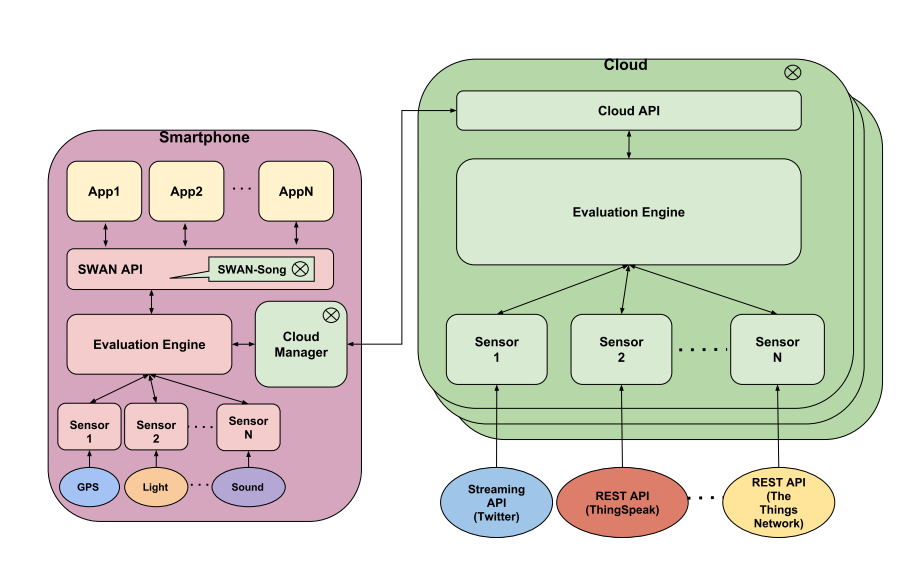
\includegraphics[width=1\textwidth]{images/cowbird_architecture.png}
 \caption{SWAN and Cowbird architecture. Cowbirds components are marked with $\otimes$. Source: \cite{cowbirdarticle}}
\label{fig:cowbird_architecture}
\end{figure}

\section{The Cowbird framework}
The Cowbird framework has been designed as a cloud extension of the SWAN framework. In particular, it enables the combination of smartphones sensors and real-time web data: these data can be originally generated by IoT sensors or, more in general, they can be any data which can be retrieved by polling a web resource (e.g. Twitter feeds) \cite{cowbirdarticle}. Furthermore, the Cowbird framework reduces the overall communication between the smartphone and the cloud in order to save energy. In fact, the evaluation of phone sensors is performed locally while the evaluation of IoT sensors is computed in the cloud.

Some core features and functionalaties of Cowbird are \cite{cowbirdarticle}:
\begin{itemize}
\item \emph{Flexibility}. The developers using the Cowbird framework
can easily connect to any cloud to offload the evaluation of the IoT sensors.
\item \emph{Usability}. Cowbird uses the SWAN-Song domain specific language to access both sensors in the phone and real-time data.
\item \emph{Portability}. The cloud part of Cowbird is programmed in
Java. Hence, it can be easily ported to any device running a JVM.
\item \emph{Privacy}. Cowbird performs the evaluation of local sensors
on the phone and evaluation of remote IoT sensors remotely. Thus, the sensitive data can be kept and processed locally on the phone.
\item \emph{Energy Efficiency}. Cowbird is designed to minimize the energy consumption of smartphones. Offloading the computation and the communication required to fetch the IoT real-time data (continuous polling from the web) to the cloud will preserve the smartphones battery life.
\item \emph{Mobile Data Cost}. Sending much data through cellular
networks is costly, so Cowbird tries to optimize the communication between the phone and the cloud. The result of the evaluation in the cloud is only sent to the phone if there is a change from the previous result. 
\end{itemize}
\subsection{Cowbird architecture details}
Cowbird enriches the SWAN framework designed to be executed on Android smartphones. In particular, Cowbird integrates novel capabilities to the existing SWAN services and it introduces new sensing services to be executed on the cloud. 

The existing SWAN framework has been extended by modifying the SWAN-Song language in order to support \emph{cloud-based expressions}. Furthermore, a new module named \emph{Cloud Manager} has been introduced: it runs on the smartphone and it is responsible for managing the communication with one or more clouds \cite{cowbirdarticle}. 

At the cloud side, the original SWAN evaluation engine has been redesigned to be executed on the cloud. The cloud side of the framework has support for various IoT sensors (implemented as virtual sensors and executed by a different thread) and a mechanism to push data to the phone.

\paragraph{}
We discuss now the typical interaction flow between Cowbird and  third-party app built on top of it. A third-party app uses the SWAN API to register a remote expression to the cloud. The expression is then sent to the evaluation engine service which will forward it to the cloud manager in the phone. The cloud manager checks the location identifier of the expression and sends it to the specified URL. The cloud acknowledges the expression and starts the evaluation by activating the relevant sensor thread. The result of the evaluation from the cloud is received by the cloud manager and is further sent to the evaluation engine in the phone for local processing. The final result is then sent back to the app.

\subsubsection{Remote expressions in Cowbird}
%	configuration app of the framework
In Cowbird, the location identifier of SWAN-Song has been extended in order to support remote expressions. The developer can add the URL of its cloud in the configuration of the SWAN framework. Then, the developer can refer to that cloud using \emph{cloud} as location identifier in its SWAN-Song expression. For example, in case of a sound sensor feed available in a certain channel of the ThingSpeak platform \cite{thingspeakonline} we can write a SWAN expression such as:
\begin{equation} \label{eq:cloudthingspeakexpression}
cloud@thingspeak:field?channelid='1'\#field='1'\big\{MEAN,20s\big\} > 50.0
\end{equation}
The expression \ref{eq:cloudthingspeakexpression} checks if the mean value over a period of 20 seconds is greater than 50.0 decibel (dB). 

The developer can also refers to the cloud indicating the endpoint directly in the SWAN-Song expression. For example, the following SWAN-Song expression perform the same evaluation of expression \ref{eq:cloudthingspeakexpression}:
\begin{dmath} \label{eq:herokuthingspeakexpression}
http://cowbird.herokuapp.com@thingspeak: field?channelid='1'\#field='1'\big\{MEAN,20s\big\} > 50.0
\end{dmath}
The SWAN-Song expression \ref{eq:herokuthingspeakexpression} assumes to have a Cowbird cloud instance running on Heroku at the URL provided as location identifier of the expression.

A combination of expressions that use smartphone local sensors (accelerometer) and IoT sensors (live data coming from ThingSpeak) can be written as:
\begin{equation}
E1 = self@movement:total\big\{ANY,1000\big\} > 15 
\end{equation}
\begin{equation}
E2 = cloud@thingspeak:field?channelid='1'\#field='1'\big\{MEAN,20s\big\} > 50.0
\end{equation}
\begin{equation} \label{eq:localcombinedexpression}
CombinedExpression = E1 \text{ \&\& } E2
\end{equation}
The evaluation of the local expression (E1) occurs locally on the Android smartphone. The evaluation of the remote expression (E2) occurs in the cloud and the result is sent to the phone. The CombinedExpression in \ref{eq:localcombinedexpression} is evaluated on the phone based on the results from E1 and E2. 

The evaluation of a SWAN-Song expression composed by two remote sub-expressions, instead, is completely evaluated in the cloud.
\begin{equation}
E1 = cloud@thingspeak:field?channelid='1' \#field='1'\big\{MEAN,200s\big\} > 50.0
\end{equation}
\begin{equation}
E2 = cloud@thingspeak:field?channelid='2' \#field='1'\big\{MEAN,200s\big\} > 50.0
\end{equation}
\begin{equation} \label{eq:remotecombinedexpression}
CombinedExpression = E1 \text{ \&\& } E2
\end{equation}

The result of the combined expression in \ref{eq:remotecombinedexpression} is evaluated on the cloud; the combined result is then sent to the phone.
\subsubsection{The Cloud Manager module}
The evaluation engine running on the smartphone registers an expression to the cloud manager using three parameters: the expression id, the expression itself and the location (URL) of the expression. The cloud manager starts a HTTP POST request to the cloud indicated by the expression with the id, expression and a Firebase token. The cloud manager runs a Firebase Message Service to receive the result of the evaluation done in the cloud. The result is received at the phone side as push notification through Firebase Cloud Messaging. 
%We chose Firebase Cloud Messaging because sensor data is typically less than 4KB (maximum payload). 
Since Cowbird is Android-based, the Google Play Service already has socket connections to the Firebase server and multiple applications can make use of this service to minimize battery consumption. The message received from the server contains the result of the expression which can be either a new value or a new TriState (TRUE, FALSE, UNDEFINED) and the expression id. The Cloud manager sends this data to the evaluation engine service for local evaluation. After the local evaluation, the final result is sent to the app.
\subsubsection{Cowbird cloud instance}
The Cowbird cloud instance is implemented using the Play Framework \cite{playframeworkonline} with Java. The Cloud API contains a controller that routes a specific URL to a functionality. The cloud instance supports requests to register expressions both from mobile clients and web clients. The Cowbird cloud instance currently supports various IoT sensors such as ThingSpeak, The Things Network, Twitter, News, Weather, Currency and Flight. Additional sensors can be easily added as a plugin. Sensors are implemented as Java threads.

On receiving a request from the phone, the Cloud API forwards it to the evaluation engine. The evaluation engine will start the relevant sensor thread that will keep polling external web data from an endpoint. The sensor data is sent back to the evaluation engine which will evaluate the data;  expression evaluation performed in a multi-threaded fashion. The evaluation result is sent to the Cloud API that will forward it to the phone.
%along with the registered token and the framework’s API key \cite{cowbirdarticle}
Communication between the Cowbird cloud instance and the phone happens through Firebase push notification.
\subsection{Cowbird communication optimization}
If the Cowbird cloud instance has to evaluate a SWAN-Song TriState expression the process of sending the result of the valuation back to the phone has been optimized. In particular, the result is sent only if there is a change in the outcome (e.g., from FALSE to TRUE), and not whenever a sensor value changes \cite{cowbirdarticle}. Minimizing the communication between the phone and the cloud reduces the energy consumption and preserves the smartphone battery life.
\section{Cowbird limitations}
The Cowbird architecture presents some limitations. In particular, the current implementation of the cloud instance does not scale since it is designed to run on a single computing node. Now imagine a scenario where many expressions from different smartphones are offloaded to the cloud; thus, many threads are instantiated in order to fetch the sensors data. Multiple running threads can easily saturate the computing resources especially if each thread performs updates with an high frequency. Furthermore, each sensor generates an unbounded and potentially infinite stream of data that has to be processed by the evaluation engine. The huge amount of data that has to be processed can overwhelm the computing resources (i.e. CPU, memory) and reduce the overall performance of the framework.

In order to evaluate the streams of data generated by the IoT sensors in real-time a distributed computing architecture is required. In the next chapters we are going to investigate how such infrastructure can be built and how the Cowbird cloud instance can be extended in order to accommodate SWAN-Song expressions evaluation on a large scale.
\clearpage{\pagestyle{empty}\cleardoublepage}
\chapter{Related work}
The internet traffic explosion started in the mid-90s induced the creation of massive datasets. Processing very large amount of data, even though can be conceptually straightforward, actually means many computations that have to be distributed across hundreds or thousands of machines in order to finish in a reasonable amount of time. In early 2000s, the developer had the burden to write complex applications responsible for parallelizing the computation, distributing the data, and handling possible failures. As a reaction to this complexity, Google in 2004 published a paper describing a novel programming model for processing large datasets named MapReduce \cite{googlemapreduce}. MapReduce provides an abstraction that allows the developer to focus on the computation he/she wants to express hiding the details of parallelization, fault-tolerance, data distribution and load balancing in a framework. The MapReduce framework takes advantage of the Google File System \cite{googlefilesystem}: a distributed file system that uses replication to provide availability and reliability on top of commodity unreliable hardware. The open source community, inspired by the Google MapReduce programming model, created Hadoop \cite{hadooponline} and HDFS \cite{hadoophdfs}. The Hadoop release boosted the growth of the big data analysis field and created new scenarios and new type of applications that were very tough to realize with previous existing tools. From that moment on, a lot of effort has been put in realizing more efficient and high-performance technologies for collecting, aggregating and analyzing huge amount of data.

In this chapter we will discuss some of the technologies and architectures that can be used in order to process large amount of data generated by (IoT) sensors, possibly in real-time.

\section{Batch-Mode architecture}
Google MapReduce and Hadoop are designed to be executed on top of clusters of computing nodes. The first releases of Hadoop integrated the cluster resource management with the data processing engine itself (Hadoop MapReduce). In 2012, Hadoop 2.0 was released \cite{hadooponline} and it introduced YARN \cite{yarn}; Apache Yet Another Resource Negotiator (YARN) decouples the programming model from the resource management infrastructure and the users' applications scheduling. In general, we can think to YARN as a distributed operating system that is capable of managing a cluster of machines and scheduling users' applications on the available resources. Furthermore, it provides an API that can be used to develop any generic distributed application. Hence, different computing frameworks that address different application requirements have been built on top of YARN (e.g. the general purpose Apache Spark \cite{apachesparkonline}, Apache Giraph \cite{apachegiraphonline} for iterative graph processing, etc.). 

 \begin{figure}[ht!]
\includegraphics[width=1\textwidth]{images/barch_architecture.pdf}
 \caption{Classic big data batch architecture}
\label{fig:batch_architecture}
\end{figure}

A big data application usually has a well defined architecture, no matter the computing framework it uses and whether or not it runs on top of YARN or on another cluster management system (e.g. Apache Mesos  \cite{apachemesosonline}, Kubernetes \cite{kubernetesonline}, in the cloud using Amazon Elastic Map Reduce (EMR) \cite{amazonemronline}). The \emph{classic} big data architecture for processing large amount of structured or unstructured data is named \emph{batch architecture} \cite{philosophydistributeddata, fastdataarchitecture, streamingbigdataprocessinginclouds}. The typical big data batch architecture consists of the following components or layers (see Figure \ref{fig:batch_architecture}):
\begin{itemize}
\item	 \emph{Data ingestion layer}. The data ingestion layer can be used to move data that can come from different sources into the persistence tier. The data ingestion layer can take advantage of special-purpose services such as Apache Flume \cite{apacheflumeonline} for log aggregation or Apache Sqoop \cite{apachesqooponline} for interoperating with databases.
\item \emph{Data persistence.} The data persistence layer is responsible of storing and indexing final as well intermediate datasets. This tier can store large amount of data using one of the next-generation database systems. In fact, the Dynamo \cite{dynamo} paper accelerated interest in NoSQL systems and many NoSQL database emerged such as Apache Cassandra \cite{apachecassandraonline} or MongoDB \cite{mongodbonline}. Furthermore, the CAP theorem emerged as a way of understanding the trade-offs between consistency and availability of service in distributed systems when a network partition occurs. For the always-on applications, it often made sense to accept \emph{eventual consistency} in exchange for a greater availability \cite{fastdataarchitecture}. In big data application, database systems are often used when row-level access (e.g. CRUD operations) is required \cite{fastdataarchitecture}.

In order to store large datasets, the data persistence layer can also use a distributed file system or object store, such as HDFS or Amazon S3 \cite{awss3online}. These systems offers lower cost per GB storage compared to databases and more flexibility for data formats \cite{fastdataarchitecture}. However, they are best used when scans are the dominant access pattern, rather than CRUD operations. 
\item  \emph{Cluster resource management}. 
\item  \emph{Data Processing.} The data analysis jobs written in Hadoop MapReduce, Spark, or other tools submitted to the cluster resource manager.
\end{itemize}

A typical big data application can be built as a \emph{workflow}, a directed graph of distributed computing jobs \cite{bigdataatlinkedin}. Each job reads one or more input datasets from the persistent storage and produces one or more output datasets. In MapReduce, if the application requires data reuse between computations (e.g. between two jobs) the intermediate result is also written to an external stable storage system. This can incur substantial overheads due to data replication, disk I/O, and serialization, which can dominate application execution times. Recognizing this problem, researchers have developed specialized frameworks for some applications that require data reuse. These frameworks only support specific computation patterns and perform data sharing implicitly for these patterns. Eventually, the general purpose computing framework Apache Spark \cite{apachespark} was released. Spark is the first system that allows a general-purpose programming language to be used at interactive speeds for in-memory data mining on clusters \cite{apachespark}. Spark is based on the concept of resilient distributed datasets (RDDs) \cite{apachesparkrdd} that enables efficient data reuse in a broad range of applications. The RDD abstraction allows users to explicitly persist intermediate results in memory, control the data partitioning to optimize the data placement, and manipulate them using a rich set of operators. Even though Spark increased the interactivity of many big data applications and tools, a typical job in batch-mode can last from few minutes to several hours. In fact, in classic batch-mode, data is collected and stored in the persistent storage layer and once in a while (e.g. every hour, once per day) the data is processed through one or more batch jobs. The high-latency imposed by the batch architecture is not suitable for real-time applications in which data should be computed as it is generated, in an incremental fashion.

\section{Real-time streaming architecture}
Recently, many big data real-time applications emerged such as detecting fraudulent financial activity as it happens or optimizing e-commerce search results in real-time. These kinds of applications process unbounded datasets and potentially infinite \emph{streams} of data, and they are often  referred as real-time streaming applications. The backbone of a real-time streaming application is usually a distributed, high-performance and always available architecture. There are many streaming systems and ways of doing streaming, and everything is evolving quickly. In this section, we will discuss and highlight the components required to build an efficient streaming architecture.




\clearpage{\pagestyle{empty}\cleardoublepage}
%\include{Architettura}
%\clearpage{\pagestyle{empty}\cleardoublepage}
%\include{TED}
%\clearpage{\pagestyle{empty}\cleardoublepage}
%!TEX encoding = UTF-8 Unicode\pagestyle{empty}
%\clearpage{\pagestyle{empty}\cleardoublepage}
%\include{APIs}
%\clearpage{\pagestyle{empty}\cleardoublepage}
%\include{Test}
%\clearpage{\pagestyle{empty}\cleardoublepage}


%%%%%%%%%%%%%%%%%%%%%%%%%%%%%%%%%%%%%%%%%non numera l'ultima pagina sinistra
\clearpage{\pagestyle{empty}\cleardoublepage}
%%%%%%%%%%%%%%%%%%%%%%%%%%%%%%%%%%%%%%%%%per fare le conclusioni
\chapter*{Conclusions and future work}
%%%%%%%%%%%%%%%%%%%%%%%%%%%%%%%%%%%%%%%%%imposta l'intestazione di pagina
%\rhead[\fancyplain{}{\bfseries
%CONCLUSIONI}]{\fancyplain{}{\bfseries\thepage}}
%\lhead[\fancyplain{}{\bfseries\thepage}]{\fancyplain{}{\bfseries
%CONCLUSIONI}}
%%%%%%%%%%%%%%%%%%%%%%%%%%%%%%%%%%%%%%%%%aggiunge la voce Conclusioni
                                        %   nell'indice
%\addcontentsline{toc}{chapter}{Conclusioni e sviluppi futuri} 
%\input{ConclusionAndFutureWorks}


 %\cite{K3,K4}.
%%%%%%%%%%%%%%%%%%%%%%%%%%%%%%%%%%%%%%%%%imposta l'intestazione di pagina
%\renewcommand{\chaptermark}[1]{\markright{\thechapter \ #1}{}}
%\lhead[\fancyplain{}{\bfseries\thepage}]{\fancyplain{}{\bfseries\rightmark}}
%\appendix                               %imposta le appendici
%\chapter{Configurazioni utilizzate nei test}               %crea l'appendice


%%%%%%%%%%%%%%%%%%%%%%%%%%%%%%%%%%%%%%%%%non numera l'ultima pagina sinistra
\printbibliography 
\clearpage{\pagestyle{empty}\cleardoublepage}
\chapter*{Acks} 
Grazie.
\end{document}
